\documentclass[a4paper]{article}

%\usepackage[utf8]{inputenc}

\usepackage{hyperref}
\usepackage{xcolor}
\usepackage{graphicx}
\usepackage[english]{babel}
\usepackage[T1]{fontenc}
\usepackage{url}
\usepackage{import}
\usepackage{multirow}
\usepackage{color}
\usepackage{fancyhdr}
\usepackage{amssymb}
\usepackage{tabu}
\usepackage{mathtools}
\usepackage[margin=2.5cm]{geometry}
\usepackage{listings}
\usepackage{titling}
\usepackage[utf8x]{inputenc}
\usepackage[numbered,framed]{matlab-prettifier}

\let\ph\mlplaceholder % shorter macro
\lstMakeShortInline"

\newcommand{\bnb}{\begin{nobreak}}
\newcommand{\enb}{\end{nobreak}}

\lstset{
  style              = Matlab-editor,
  basicstyle         = \mlttfamily,
  escapechar         = ",
  mlshowsectionrules = true,
}

\pretitle{%
  \begin{center}
  \LARGE
  
\includegraphics[width=\textwidth/4]{assets/logo-unifi.png}\\[\bigskipamount]
}
\posttitle{\end{center}}
\date{}

\begin{document}



\title{\vspace{2cm}Elaborato di\\ \textbf{Calcolo Numerico}\\ Anno Accademico 2017/2018\vspace{3cm}}

\author
{Yuri \emph{Bacciarini} - \texttt{5530804} - {\textit{yuri.bacciarini@stud.unifi.it}}}

\maketitle
\newpage
\tableofcontents


\newpage
\section{\textbf{Capitolo 1}}
\section{\textbf{Capitolo 1}}
\subsection{Esercizio 1}
Volendo conoscere quanto un errore influenzi il risultato quando $x\neq0$, si definisce l’errore relativo:
\[
|\epsilon_x| = \frac{\tilde{x}-x}{x} 
\]
da cui :
\[
\tilde{x} = x(1+\epsilon_x), \text{ e quindi } \frac{\tilde{x}}{x} = 1 + \epsilon_x
\]
ovvero l’errore relativo deve essere comparato a 1: un errore relativo vicino a zero indicherà che il risultato approssimato è molto vicino al risultato esatto,mentre un errore relativo uguale a 1 indicherà la totale perdita di informazione.\\\\
Con $x = e \approx 2.7183 = \tilde{x}, \text{l'errore relativo è quindi } |\epsilon_x| = \frac{2.7183 - e}{e} = 6.6849e-06$\\\\
Il numero di cifre significative \textit{k} corrette all’interno di $\tilde{x}$ si definisce con la formula :
\[
\textit{k} = -\log(2|\epsilon_x|)
\]
In questo caso il risultato del calcolo è $\textit{k}=4.8739$, che è abbastanza vicino alla realtà di $\textit{k}=5$ cifre significative corrette.\\\\
Spesso, per avere un’idea di quanto è l’ordine di grandezza di $\epsilon$ si scrive:
\[
|\epsilon_x| \approx \frac{1}{2}10^{-\textit{k}}
\]
infatti : 
\[
|\epsilon_x| \approx \frac{1}{2}10^{-4.8739} = 6.6849e-06 = |\epsilon_x|
\]
\subsection{Esercizio 2}
Partiamo da :
	\[
	f'(x) \approx \frac{f(x+h) - f(x-h)}{2h}
	\]
Usando gli sviluppi di Taylor fino al secondo ordine otteniamo:
	\[
	f(x+h) = f(x) + f'(x)h + \frac{1}{2} f''(x)h^{2} + \frac{1}{6}f'''(\xi_x)h^{3}
	\]
	\[f(x-h) = f(x) - f'(x)h + \frac{1}{2} f''(x)h^{2} - \frac{1}{6}f'''(\mu_x)h^{3}
	\]
Al numeratore otteniamo
	\[
	f(x+h) - f(x-h) = 2f'(x)h + \frac{1}{6}(f'''(\xi_x)h^{3}+f'''(\mu_x)h^{3})
	\]
La relazione iniziale diventa
	\[
	f'(x) \approx \frac{f(x+h) - f(x-h)}{2h} - \frac{1}{12}(f'''(\xi_x) + f'''(\mu_x))h^{2}
	\]
Abbiamo quindi verificato, usando gli sviluppi di Taylor fino al secondo ordine con resto in forma di Lagrange, se f $\in C^{3}$ risulta
	\[
	f'(x) = \phi_h(x) + O(h^2)
	\]
dove
	\[
	\phi_h(x) = \frac{f(x+h) - f(x-h)}{2h}
	\]
\subsection{Esercizio 3}
Il seguente codice MatLab, riguarda la funzione $\theta_{h}(x) = \frac{f(x+h)-f(x-h)}{2h}$, indicando con $h=10^-j$, $j=1,...,10$, $f(x)=x^4$ e $x=1$ :\\
	\lstinputlisting[language=Matlab]{Cap_1/Es_3/Es_3.m}
restituisce i seguenti valori:\\
\begin{center}
	\begin{tabular}{|c|c|}
		\hline
			$h$ & $\theta_{h}(1)$  \\
		\hline
    		\(10^{-1}\) & $4.040000000000002e+00$\\
    		\(10^{-2}\) & $4.000400000000004e+00$\\
    		\(10^{-3}\) & $4.000003999999723e+00$\\
    		\(10^{-4}\) & $4.000000039999230e+00$\\
    		\(10^{-5}\) & $4.000000000403681e+00$\\
    		\(10^{-6}\) & $3.999999999948489e+00$\\
    		\(10^{-7}\) & $4.000000000115023e+00$\\
    		\(10^{-8}\) & $4.000000003445692e+00$\\
    		\(10^{-9}\) & $4.000000108916879e+00$\\
    		\(10^{-10}\) & $4.000000330961484e+00$\\
		\hline
	\end{tabular}
\end{center} 
Si vede che i valori di $\theta_{h}(1)$ diminuiscono fino ad $h = 10^{-6}$, in cui si ha il minimo valore di $\theta_{h}(1)$, dopodichè inizia a crescere. Mostriamo l'andamento relativo nel seguente plot:
\begin{figure}[H]
	\label{Cap_1_Es_3}
	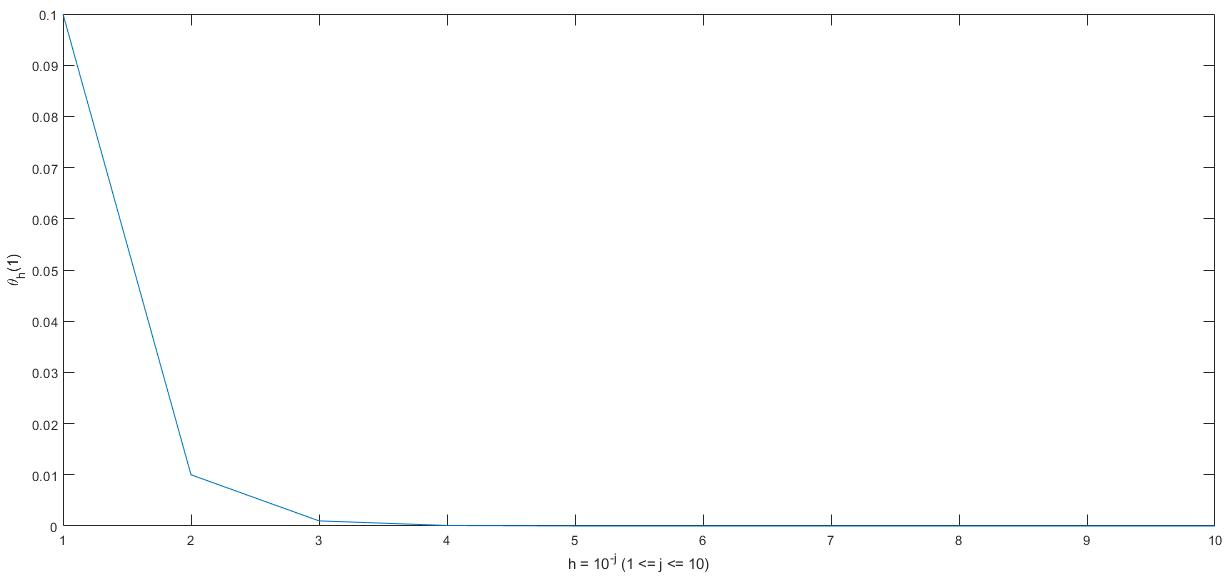
\includegraphics[width=\textwidth]{Plot/Cap_1_Es_3}
		\caption{Andamento della funzione $\theta_{h}(1)$}
\end{figure}
\subsection{Esercizio 4}
Le due espressioni in aritmetica finita vengono scritte tenendo conto dell'errore di approssimazione sul valore reale:\\
\begin{enumerate}
	\item $(x \oplus y) \oplus z \equiv fl(fl(fl(x)+fl(y))+fl(z)) = ((x(1+\varepsilon_{x})+y(1+\varepsilon_{y}))(1+\varepsilon_{a})+z(1+\varepsilon_{z}))(1+\varepsilon_{b})$
	\item $x \oplus (y \oplus z) \equiv fl(fl(x)+fl(fl(y)+fl(z))) = (x(1+\varepsilon_{x})+(y(1+\varepsilon_{y})+z(1+\varepsilon_{z}))(1+\varepsilon_{a}))(1+\varepsilon_{b})$\\
\end{enumerate}
Indichiamo con $\varepsilon_{x},\varepsilon_{y},\varepsilon_{z}$ i relativi errori di $x, y, z$ e con $\varepsilon_{a},\varepsilon_{b}$ gli errori delle somme e per calcolare l'errore relativo delle due espressioni consideriamo $\varepsilon_{m} = max\{|\varepsilon_{x}|,|\varepsilon_{y}|,|\varepsilon_{z}|,|\varepsilon_{a}|,|\varepsilon_{b}|\}$.\\
Dalla definizione di errore relativo si ha quindi:\\
\begin{enumerate}
    \item 
   		\[
    		\varepsilon_{1} = \frac{((x(1+\varepsilon_{x})+y(1+\varepsilon_{y}))(1+\varepsilon_{a})+z(1+\varepsilon_{z}))(1+\varepsilon_{b})-(x+y+z)}{x+y+z} \approx
    	\]
    	\[
    		\approx \frac{x(1+\varepsilon_{x}+\varepsilon_{a}+\varepsilon_{b})+y(1+\varepsilon_{y}+\varepsilon_{a}+\varepsilon_{b})+z(1+\varepsilon_{z}+\varepsilon_{b})-x-y-z}{x+y+z} \leq
    	\]
    	\[ 
    		\leq\left|\frac{\varepsilon_{b}(x+y+z)+\varepsilon_{a}(x+y)+x\varepsilon_{x}+y\varepsilon_{y}+z\varepsilon_{z}}{(x+y+z)}\right|\leq
    	\]
    	\[
    		\leq\frac{|\varepsilon_{b}||x+y+z|+|\varepsilon_{a}||x+y|+|x||\varepsilon_{x}|+|y||\varepsilon_{y}|+|z||\varepsilon_{z}|}{|x+y+z|}\leq
    	\]
    	\[
    		\leq\varepsilon_{m}\frac{|x+y+z|+|x+y|+(|x|+|y|+|z|)}{|x+y+z|}=
    	\]
    	\[
    		=\varepsilon_{m}\left(1+\frac{|x+y|}{|x+y+z|}+\frac{|x|+|y|+|z|}{|x+y+z|}\right)
    	\]\\\
    \item Tenendo presente che $x \oplus (y \oplus z) = (y \oplus z) \oplus x$, seguendo gli stessi procedimenti del punto precedente possiamo scrivere:\\
    	\[
    		\varepsilon_{2} = \frac{((y(1+\varepsilon_{y})+z(1+\varepsilon_{z}))(1+\varepsilon_{a})+x(1+\varepsilon_{x}))(1+\varepsilon_{b})-(y+z+x)}{y+z+x} \approx
    	\]
    	\[
    		\approx \frac{y(1+\varepsilon_{y}+\varepsilon_{a}+\varepsilon_{b})+z(1+\varepsilon_{z}+\varepsilon_{a}+\varepsilon_{b})+x(1+\varepsilon_{x}+\varepsilon_{b})-y-z-x}{y+z+x} \leq
    	\]
    	\[ 
    		\leq\left|\frac{\varepsilon_{b}(y+z+x)+\varepsilon_{a}(y+z)+y\varepsilon_{y}+z\varepsilon_{z}+x\varepsilon_{x}}{(y+z+x)}\right|\leq
    	\]
    	\[
    		\leq\frac{|\varepsilon_{b}||y+z+x|+|\varepsilon_{a}||y+z|+|y||\varepsilon_{y}|+|z||\varepsilon_{z}|+|x||\varepsilon_{x}|}{|y+z+x|}\leq
    	\]
    	\[
    		\leq\varepsilon_{m}\frac{|y+z+x|+|y+z|+(|y|+|z|+|x|)}{|y+z+x|}=
    	\]
    	\[
    		=\varepsilon_{m}\left(1+\frac{|y+z|}{|y+z+x|}+\frac{|y|+|z|+|x|}{|y+z+x|}\right)
    	\]\\\
\end{enumerate}
Otteniamo quindi che i valori degli errori $\varepsilon_{1}$ e $\varepsilon_{2}$ sono condizionati rispettivamente, dai valori $\frac{|x+y|}{|x+y+z|}$ e $\frac{|y+z|}{|y+z+x|}$.
\subsection{Esercizio 5}
Il seguente codice MatLab:\\
\lstinputlisting[language=Matlab]{Cap_1/Es_5/Es_5.m}
restituisce i seguenti valori:\\
\begin{enumerate}
\item $delta = 1/16$\\
Il valore di $delta=[0.0625]_{10}$ in binario si scrive $delta=[0,0001]_2$ . Al passo 16, che sarà il valore di \textit{count} la rappresentazione di $x$ sarà uguale a 1, e siccome l'unica condizione di uscita dello while è $x~=1$, il ciclo si arresterà.
\\
\item $delta = 1/20$\\
Il valore di $delta=[0,05]_{10}$ in binario si scrive $delta=[0,00\overline{0011}]_2$ . A differenza del caso precedente, si può notare che la rappresentazione del valore di delta in binario è periodica. Al passo 10 la rappresentazione di $x$ sarà diversa da 1, poichè la somma riguarda numeri periodici, e siccome l'unica condizione di uscita dello while è $x~=1$, il ciclo non si arresterà mai.\\
Possiamo provarlo effettuando la somma in binario di:
\[
\Big[\frac{1}{20}\Big]_{10}=\Big[0,00\overline{0011}\Big]_2
\]
\[
\Big[0,00\overline{0011}\Big]_2+\Big[0,00\overline{0011}\Big]_2+ \underbrace{...}_{6 volte}+\Big[0,00\overline{0011}\Big]_2+\Big[0,00\overline{0011}\Big]_2 = 
\]
\[
= [0.100011]_2 \approx [0.546875]_{10} \neq [1.00000]_{10}
\]
che spiegherebbe il motivo del loop dello while.
\end{enumerate}
\subsection{Esercizio 6}
\begin{enumerate}
	\item
		Il seguente codice MatLab, riguarda la prima successione $x_{k+1} = (x_k + 3/x_k)/2$, indicando con $x=x_k$, $r=\epsilon$ e $conv = \sqrt{3} \approx 1.73205080756888e+000$ :\\
		\lstinputlisting[language=Matlab]{Cap_1/Es_6/FirstSucc.m}
		restituisce i seguenti valori:\\
		\begin{center}
			\begin{tabular}{|c|c|c|}
			\hline
				$k$ & $x_k$ & $\epsilon_k$ \\
			\hline
    			$k=0$ & $x_0 = 3.00000000000000e+000$ & $\epsilon_0 = 1.26794919243112e+000$\\
    			$k=1$ & $x_1 = 2.00000000000000e+000$ & $\epsilon_1 =  267.949192431123e-003$\\
    			$k=2$ & $x_2 = 1.75000000000000e+000$ & $\epsilon_2 = 17.9491924311228e-003$\\
    			$k=3$ & $x_3 = 1.73214285714286e+000$ & $\epsilon_3 = 92.0495739800131e-006$\\
    			$k=4$ & $x_4 = 1.73205081001473e+000$ & $\epsilon_4 = 2.44585018904786e-009$\\
    			$k=5$ & $x_5 = 1.73205080756888e+000$ & $\epsilon_5 = 0.00000000000000e+000$\\
			\hline
			\end{tabular}
		\end{center}
		I calcoli indicano che per valori di $k$ superiori a 4, l'errore assoluto indicato con $\epsilon$, è dell'ordine di \(10^{-9}\), cioè $\leq$ \(10^{-12}\).\\
	\item
		Il seguente codice MatLab, riguarda la seconda successione $x_{k+1} = (3+x_{k-1}x_k)/(x_{k-1}x_k)$, indicando con $x=x_k$, $r=\epsilon$ e $conv = \sqrt{3} \approx 1.73205080756888e+000$ :\\
		\lstinputlisting[language=Matlab]{Cap_1/Es_6/SecondSucc.m}
		restituisce i valori:\\
		\begin{center}
			\begin{tabular}{|c|c|c|}
			\hline
				$k$ & $x_k$ & $\epsilon_k$ \\
			\hline
    			$k=0$ & $x_0 = 3.00000000000000e+000$ & $\epsilon_0 = 1.26794919243112e+000$\\
    			$k=1$ & $x_1 = 2.00000000000000e+000$ & $\epsilon_1 = 267.949192431123e-003$\\
    			$k=2$ & $x_2 = 1.80000000000000e+000$ & $\epsilon_2 = 67.9491924311229e-003$\\
    			$k=3$ & $x_3 = 1.73684210526316e+000$ & $\epsilon_3 = 4.79129769428077e-003$\\
    			$k=4$ & $x_4 = 1.73214285714286e+000$ & $\epsilon_4 = 92.0495739797911e-006$\\
    			$k=5$ & $x_5 = 1.73205093470604e+000$ & $\epsilon_5 = 127.137164351865e-009$\\
    			$k=6$ & $x_6 = 1.73205080757226e+000$ & $\epsilon_6 = 3.37863070853928e-012$\\
    			$k=7$ & $x_7 = 1.73205080756888e+000$ & $\epsilon_7 = 222.044604925031e-018$\\
			\hline
			\end{tabular}
		\end{center}
		I calcoli indicano che per valori di $k$ superiori a 6 incluso, l'errore assoluto indicato con $\epsilon$, è dell'ordine di \(10^{-12}\), cioè $\leq$ \(10^{-12}\).\\
\end{enumerate}


\newpage
\section{\textbf{Capitolo 2}}
\subsection{\textbf{Esercizio 2.1}}
blablabla

\newpage
\section{\textbf{Capitolo 3}}
\subsection{\textbf{Esercizio 3.1}}
\lstinputlisting[language=Matlab]{cap_3/es1/es1.m}
\lstinputlisting[language=Matlab]{cap_3/es1/triangolareInferiore.m}

Esempio: 
\begin{bmatrix}
	1 & 2 & 0 \\ 
	2 & 1 & 0 \\
	2 & 2 & 1 
\end{bmatrix}
x =
\begin{bmatrix}
  2 \\
  2 \\
  2
\end{bmatrix}

restituisce il seguente vettore
x =
\begin{bmatrix}
  2 \\
  -2 \\
  2
\end{bmatrix}
\subsection{\textbf{Esercizio 3.2}}
Fattorizzazione LDL^{t}

\lstinputlisting[language=Matlab]{cap_3/es2/es2.m}
\lstinputlisting[language=Matlab]{cap_3/es2/fattorizzazioneLDLt.m}

La matrice {A_1} = 

\begin{bmatrix}
	1  & -1  & 2   & 2  \\ 
	-1 & 5   & -14 & 2  \\
	2  & -14 & 42  & 2  \\
	2  & 2   & 2   & 65 
\end{bmatrix}

è fattorizzabile LDL^t, è quindi sdp.

La matrice {A_2} = 
\begin{bmatrix}
	1  & -1  & 2   & 2   \\ 
	-1 & 6   & -17 & 3   \\
	2  & -17 & 48  & -16 \\
	2  & 3   & -16 & 4   
\end{bmatrix}

non è fattorizzabile LDL^t, quindi non è sdp.
\subsection{\textbf{Esercizio 3.3}}
Risoluzione A x = b con A in formato LDL^t

\lstinputlisting[language=Matlab]{cap_3/es3/risolutoreLDLt.m}
\lstinputlisting[language=Matlab]{cap_3/es3/scomponiLDLt.m}
\lstinputlisting[language=Matlab]{cap_3/es3/diagonale.m}
\subsection{\textbf{Esercizio 3.4}}
Risoluzione A x = b con A in formato LU

\lstinputlisting[language=Matlab]{cap_3/es4/risolutoreLUP.m}
\lstinputlisting[language=Matlab]{cap_3/es4/scomponiLU.m}
\lstinputlisting[language=Matlab]{cap_3/es4/triangolareSuperiore.m}
\subsection{\textbf{Esercizio 3.5}}
\lstinputlisting[language=Matlab]{cap_3/es5/es5.m}

\begin{flushleft}
	\textbf{Esempio risolutoreLDL^t}
	
	Esempio: 
	A = 
	\begin{bmatrix}
		1 & 3   & 4    \\ 
		3 & 1   & -60  \\
		4 & -60 & -640 
	\end{bmatrix}
	x =
	\begin{bmatrix}
		1 \\
		2 \\
		3 
	\end{bmatrix}
	
	Dove A = LDL^t
	
	L = 
	\begin{bmatrix}
		1 & 0 & 0 \\ 
		3 & 1 & 0 \\
		4 & 9 & 1 
	\end{bmatrix}
	
	D = 
	\begin{bmatrix}
		1 & 0  & 0  \\ 
		0 & -8 & 0  \\
		0 & 0  & -8 
	\end{bmatrix}
	
	
	L^t = 
	\begin{bmatrix}
		1 & 3 & 4 \\ 
		0 & 1 & 9 \\
		0 & 0 & 1 
	\end{bmatrix}
	
	Il risultato ottenuto di x è
	\begin{bmatrix}
		-22.3750000000000 \\
		9.12500000000000  \\
		-1                
	\end{bmatrix}
	
\end{flushleft}
\begin{flushleft}
	\textbf{Esempio risolutoreLUP}
	
	Esempio: 
	A = 
	\begin{bmatrix}
		2 & 4 & 9 \\ 
		6 & 5 & 6 \\
		8 & 2 & 9 
	\end{bmatrix}
	xx =
	\begin{bmatrix}
		1 \\
		2 \\
		3 
	\end{bmatrix}
	
	Dove A = LU
	L = 
	\begin{bmatrix}
		1 & 0 & 0 \\ 
		6 & 1 & 0 \\
		8 & 2 & 1 
	\end{bmatrix}
	
	U = 
	\begin{bmatrix}
		2 & 4 & 9 \\ 
		0 & 5 & 6 \\
		0 & 0 & 9 
	\end{bmatrix}
	
	P = 
	\begin{bmatrix}
		1 & 0 & 0 \\ 
		0 & 1 & 0 \\
		0 & 0 & 1 
	\end{bmatrix}
	
	Il risultato ottenuto di xx è
	\begin{bmatrix}
		1.40000000000000  \\
		-1.20000000000000 \\
		0.333333333333333 
	\end{bmatrix}
	
\end{flushleft}

\begin{tabular}{ | l | c | r | }
	\hline
	K(A)    & ||R||/||b|| & \[\frac{||x-\widetilde{x}||}{||\widetilde{x}||}\] \\
	\hline
	nero    & 0           & zero                                          \\
	marrone & 1           & uno                                           \\
	rosso   & 2           & due                                           \\
	arancio & 3           & tre                                           \\
	giallo  & 4           & quattro                                       \\
	verde   & 5           & cinque                                        \\
	blu     & 6           & sei                                           \\
	viola   & 7           & sette                                         \\
	\hline
\end{tabular}

\pagenumbering{roman}

\end{document}
